\subsection{VGG Network}
\label{appendix:vgg_network}

The VGG architecture was introduced in a 2014 paper \cite{vgg16} titled "Very deep convolutional networks for large-scale image recognition". In it, the authors proposed a deep convolutional neural network architecture that achieved state-of-the-art results on the ImageNet dataset. The VGG architecture is characterized by its simplicity, with only 3x3 convolutional layers and 2x2 pooling layers. The VGG architecture is widely used in computer vision tasks, including image classification, object detection, and image segmentation, even to this day.


\begin{figure}
    \centering
    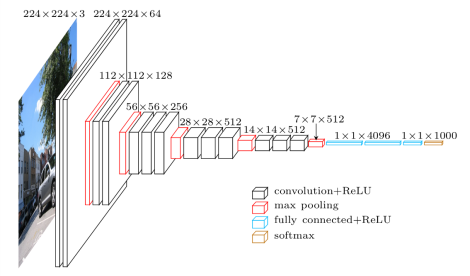
\includegraphics[width=0.6\textwidth]{images/appendix/vgg.png}
    \caption{The VGG architecture. Image credit goes to: \href{https://paperswithcode.com/method/vgg}{Code with Papers} }
\end{figure}


\begin{lstlisting}[language=Python, caption=Simple PyTorch implementation of the VGG network. Credit goes to: \href{https://github.com/pytorch/vision/tree/6db1569c89094cf23f3bc41f79275c45e9fcb3f3/torchvision/models}{pytorch github page}.]
    self.classifier = nn.Sequential(
            nn.Linear(512 * 7 * 7, 4096),
            nn.ReLU(True),
            nn.Dropout(),
            nn.Linear(4096, 4096),
            nn.ReLU(True),
            nn.Dropout(),
            nn.Linear(4096, num_classes),
        )
\end{lstlisting}
